\chapter{Materials and Methods} \label{chap:2}

\begin{figure}[!hbt]
    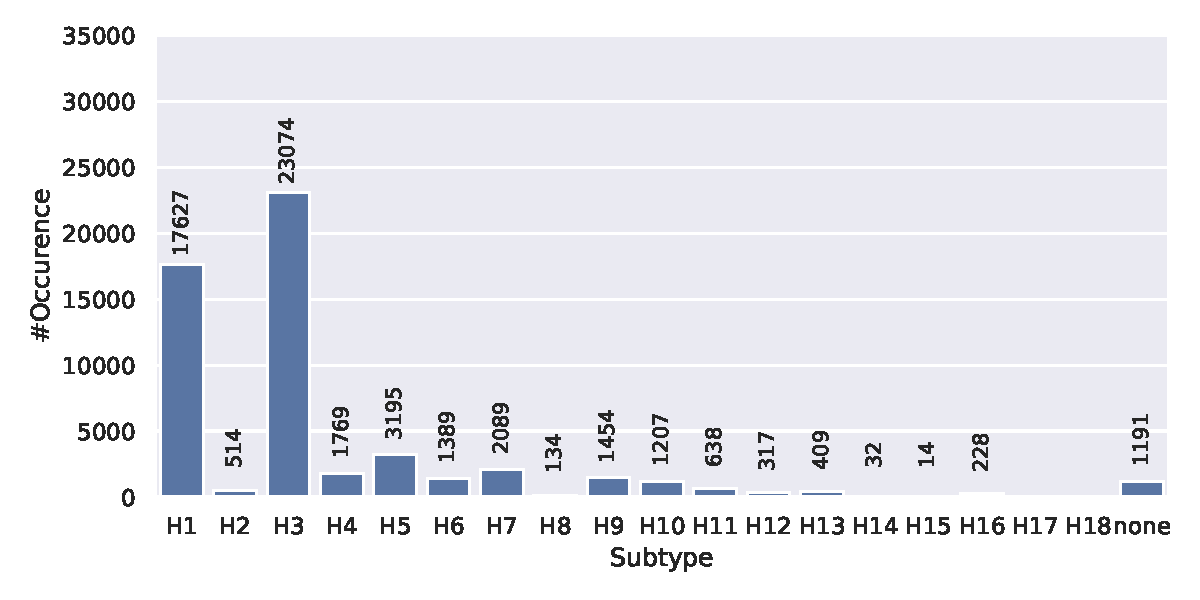
\includegraphics[width=\dimexpr\textwidth-2\fboxsep-2\fboxrule,fbox]{PCA/Data_Overview_Segment_4_H.pdf}
    \caption[Segment 4 \Acrlong{HA} Antigen Subtype Frequency]{\textbf{Segment 4 \Acrlong{HA} Antigen Subtype Frequency.} .}
    \label{fig:2.0.1}
\end{figure}

\begin{figure}[!hbt]
    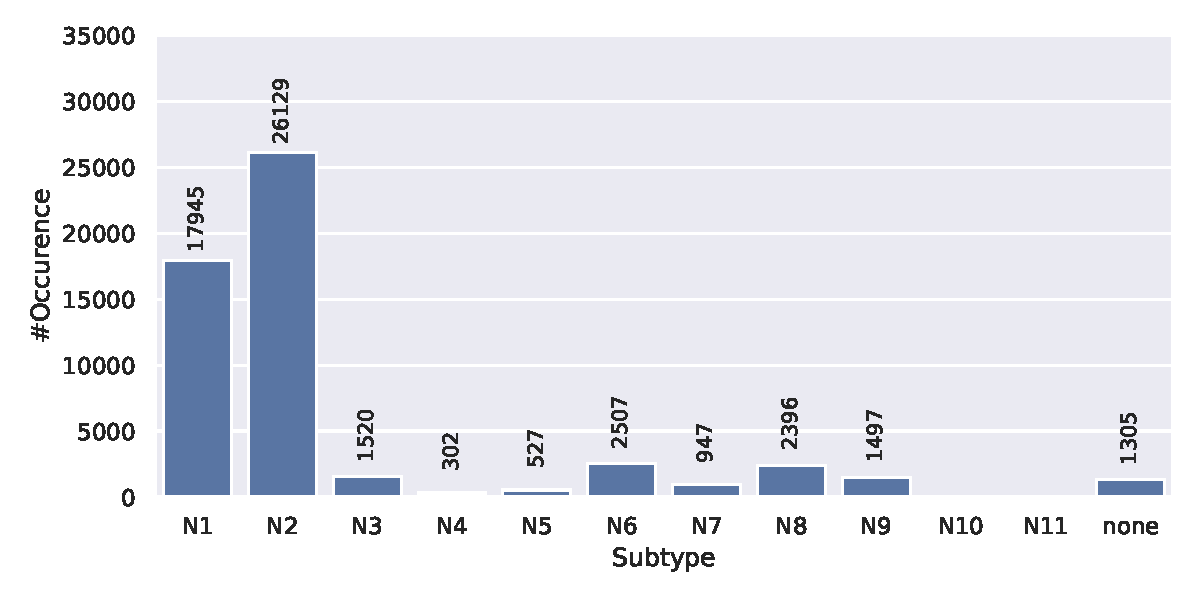
\includegraphics[width=\dimexpr\textwidth-2\fboxsep-2\fboxrule,fbox]{PCA/Data_Overview_Segment_6_N.pdf}
    \caption[Segment 6 \Acrlong{NA} Antigen Subtype Frequency]{\textbf{Segment 4 \Acrlong{NA} Antigen Subtype Frequency.} .}
    \label{fig:2.0.2}
\end{figure}

\section{Pipeline} \label{sec:2.1}

\blindtext

\section{PCA} \label{sec:2.2}

\blindtext

\section{UMAP} \label{sec:2.3}

\blindtext

\section{L2 Normalization} \label{sec:2.4}

\blindtext

\begin{figure}[!hbt]
    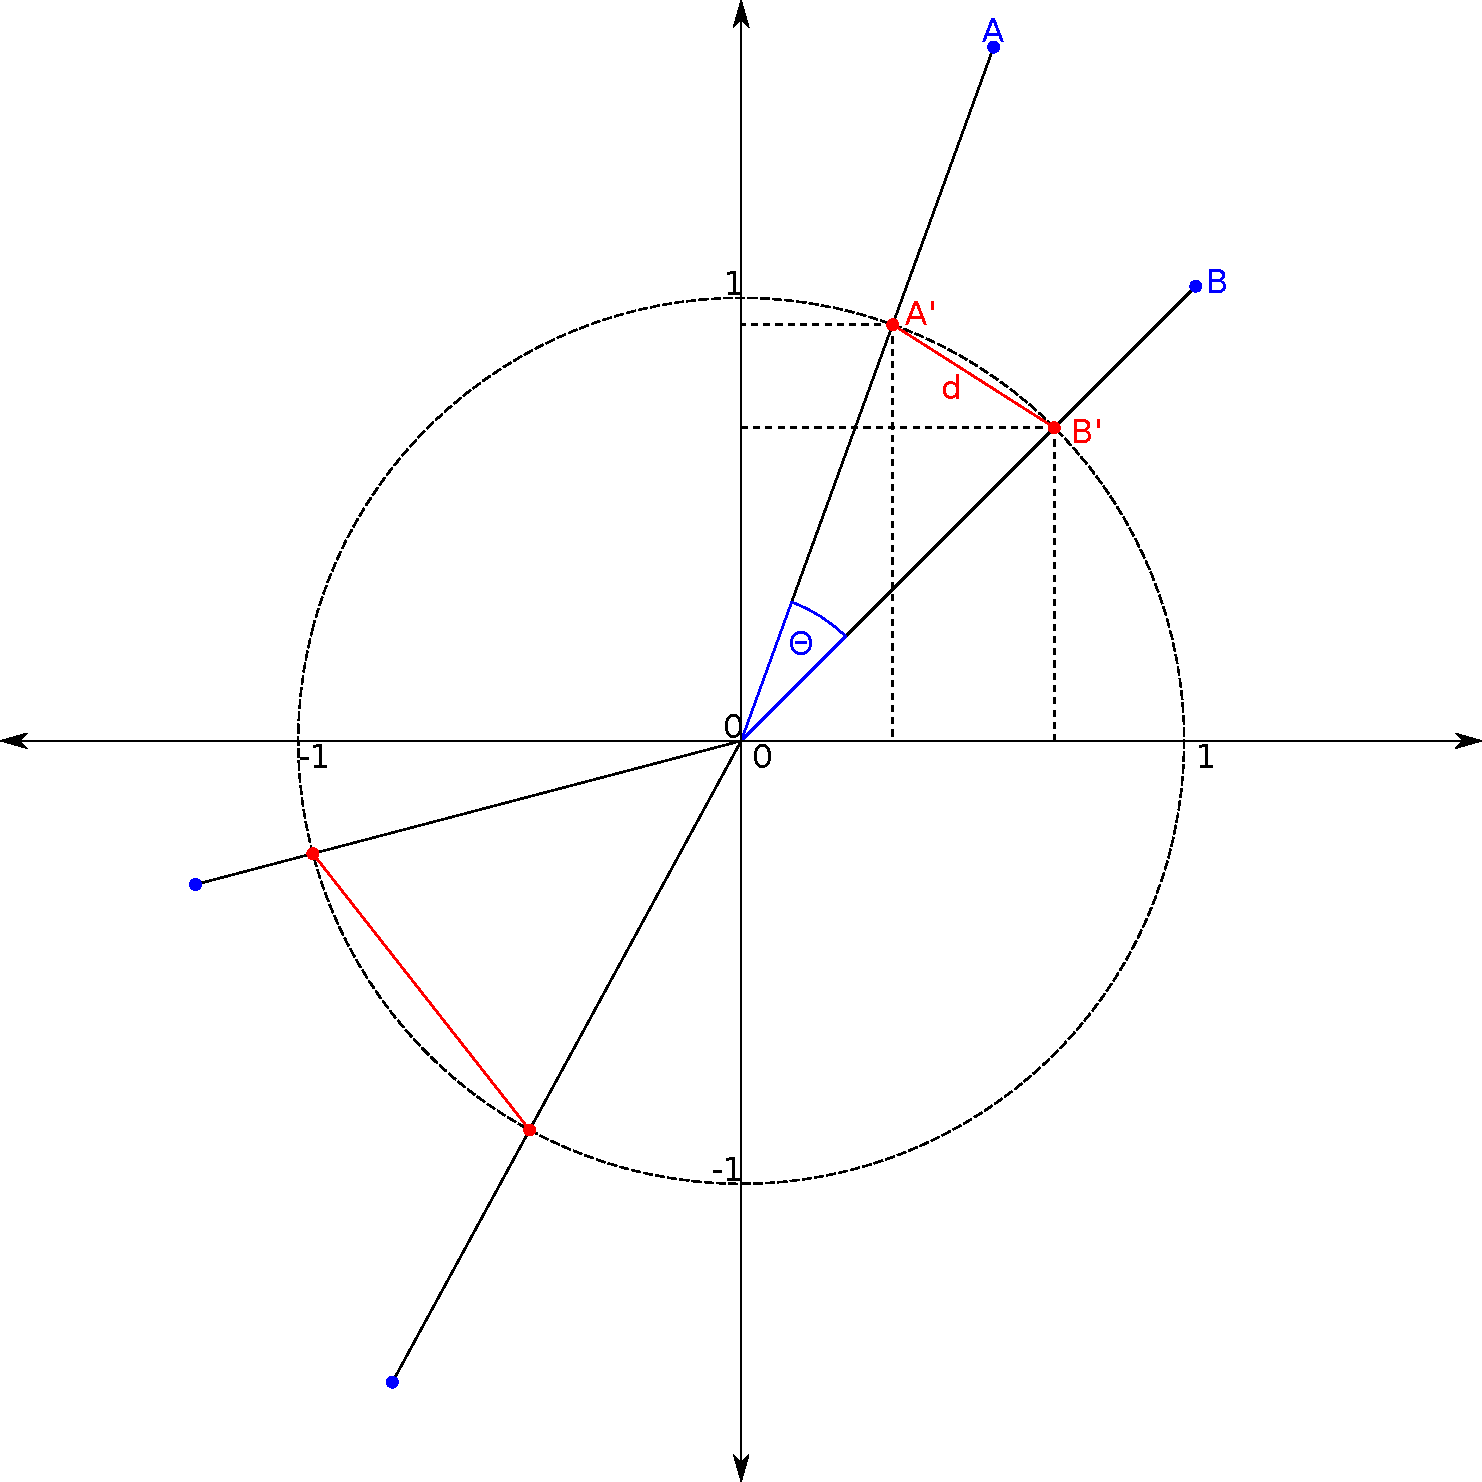
\includegraphics[width=\dimexpr\textwidth-2\fboxsep-2\fboxrule,fbox]{Extra_Graphics/L2_Euclidean.pdf}
    \caption[Cosine Distance Approximation with L2 Normalisation]{\textbf{Cosine Distance Approximation with L2 Normalisation.} .}
    \label{fig:2.4.1}
\end{figure}

\begin{figure}
    \begin{adjustbox}{minipage=\dimexpr\textwidth-2\fboxsep-2\fboxrule,fbox}
        \begin{subfigure}[b]{0.475\textwidth}
            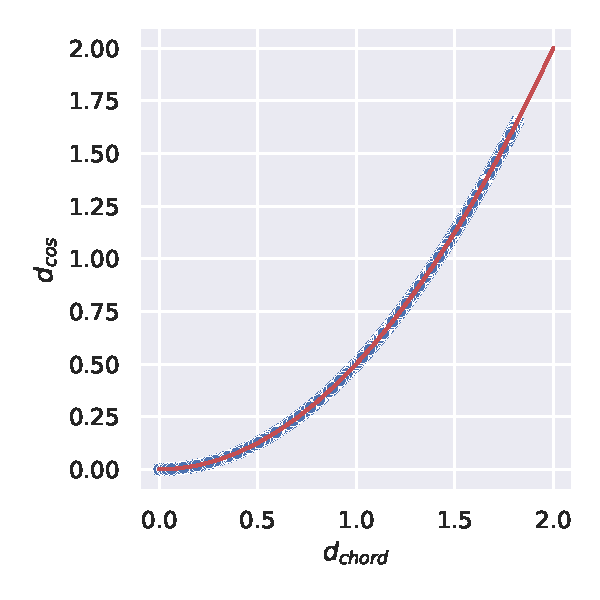
\includegraphics[width=\textwidth]{PCA/Difference_Distance_Calculation.pdf}
            \caption[Dimension Reduction with PCA]{\textbf{Dimension Reduction with PCA}}
            \label{fig:2.4.2a}
        \end{subfigure}
        \hfill
        \begin{subfigure}[b]{0.475\textwidth}
            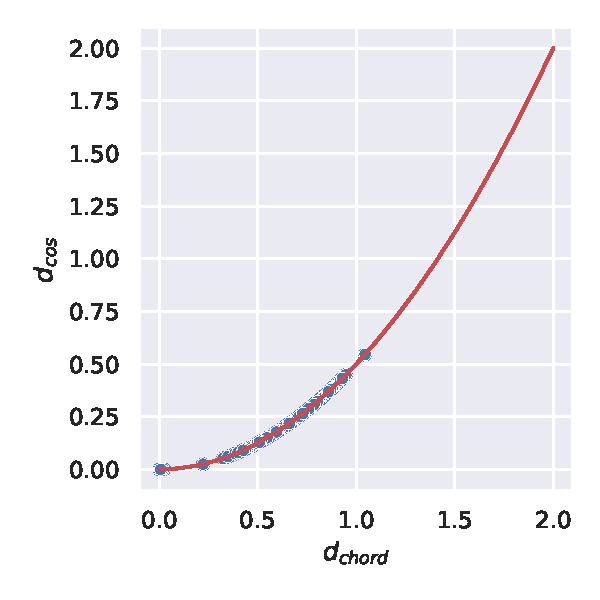
\includegraphics[width=\textwidth]{UMAP/Difference_Distance_Calculation.pdf}
            \caption[Dimension Reduction with UMAP]{\textbf{Dimension Reduction with UMAP}}
            \label{fig:2.4.2b}
        \end{subfigure}
    \end{adjustbox}
    \caption[Approximation after Dimension Reduction]{\textbf{Approximation after Dimension Reduction.} .}
    \label{fig:2.4.2}
\end{figure}

\section{Hierarchical Density-Based Spatial Clustering of Applications with Noise} \label{sec:HDBSCAN}

\gls{HDBSCAN} was used to cluster the reduced vectors \autoref{fig:Clustering_Pipeline} \textsf{\textbf{F}}). It is an clustering algorithm proposed by \textcite{campello_hierarchical_2015} as a novel version of the well-known \gls{DBSCAN} \autocite{hutchison_density-based_2013}. Execution of \gls{HDBSCAN} involves varying values of $\varepsilon$, thus, not one specific threshold is used to define the clusters, but instead clusters of varying densities are extracted based on their stability over epsilon \autocite{mcinnes_hdbscan_2017}. 

As proposed in \textcite{malzer_hybrid_2020}, by combining \gls{HDBSCAN} with \gls{DBSCAN}, some of the disadvantages of using either of these methods can be avoided \autocite{mcinnes_hdbscan_2017, moulavi_density-based_2014}. Since \gls{DBSCAN} is a hierarchical clustering tool, it is dependent on a strict threshold for clustering. Points not included in this threshold value are omitted and not clustered \autocite{ester_density-based_1996, schubert_dbscan_2017}. \gls{HDBSCAN}, on the other hand, tend to create unwanted micro-clusters in areas of high density \autocite{mcinnes_hdbscan_2017}. Using the hybrid approach proposed in \autocite{malzer_hybrid_2020}, a threshold value $\varepsilon$ can be used to extract these high density areas as single clusters with \gls{DBSCAN}, but still use the method of \gls{HDBSCAN} for the otherwise omitted points (\autoref{fig:Hybrid}). This method is useful when having a small cluster size value, while still aiming to cluster high-density areas together exactly suitable for the proposed clustering. Specific strains of \gls{IAV} are sequenced a lot more, thereby probably creating high-density areas that should be clustered together with \gls{DBSCAN}. The small cluster size is, thereby, used to find small clusters of rare sequenced variants by \gls{HDBSCAN}, with possibly important mutations in low-density areas \autocite{malzer_hybrid_2020}. As explained, the smallest minimum cluster size of 2 was used to capture, in the best case, even genomes with single \glspl{SNP} at rare appearing positions, in their own clusters. To declare as least points as possible as noise, the minimum samples value was also set to the minimum 1. 

Distance calculations by \gls{HDBSCAN} were performed with the euclidean distance setting due to an open issue in the GitHub Repository of \gls{HDBSCAN}\footnote{\url{https://github.com/scikit-learn-contrib/hdbscan/issues/69 (last accessed 06/02/21)}}. In the issue the inability to use cosine distance metric with \gls{HDBSCAN} and the approximation of it by chord distance metric, was described. Given that chord distance metric is also not available firsthand, it was also mentioned, that it can be used by normalization of the dataset with L2-norm, prior to clustering with euclidean metric setting \autoref{fig:Clustering_Pipeline} \textsf{\textbf{E}}). 

\begin{figure}[!hbt]
    \centering
    \begin{subfigure}[b]{0.475\textwidth}
        \caption[Chord]{\textbf{Chord}}
        \label{subfig:Chord}
        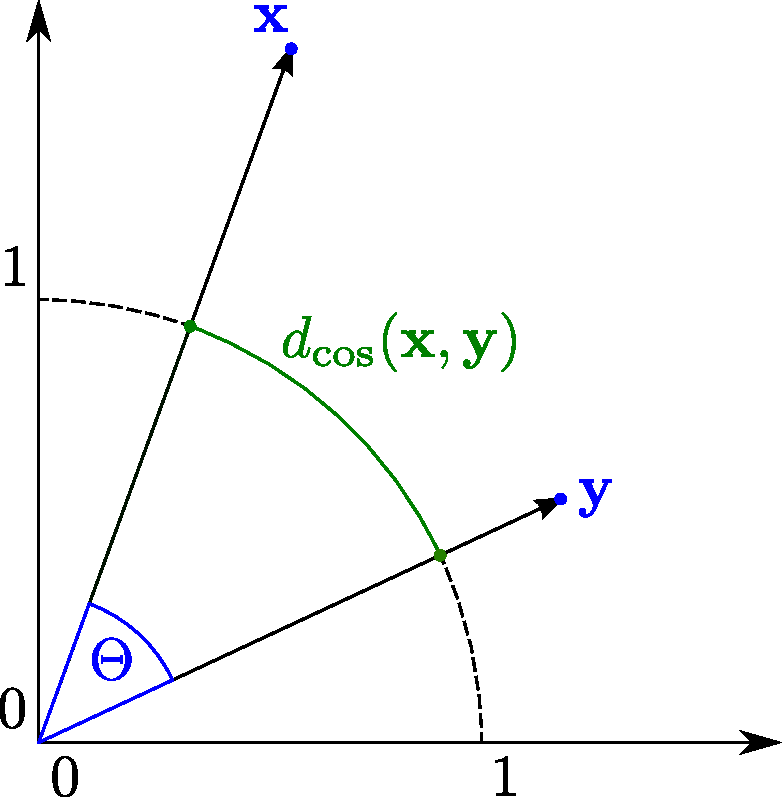
\includegraphics[width=\textwidth]{Graphics/Chord.pdf}
    \end{subfigure}
    \hfill
    \begin{subfigure}[b]{0.475\textwidth}
        \caption[L2]{\textbf{L2}}
        \label{subfig:L2}            
        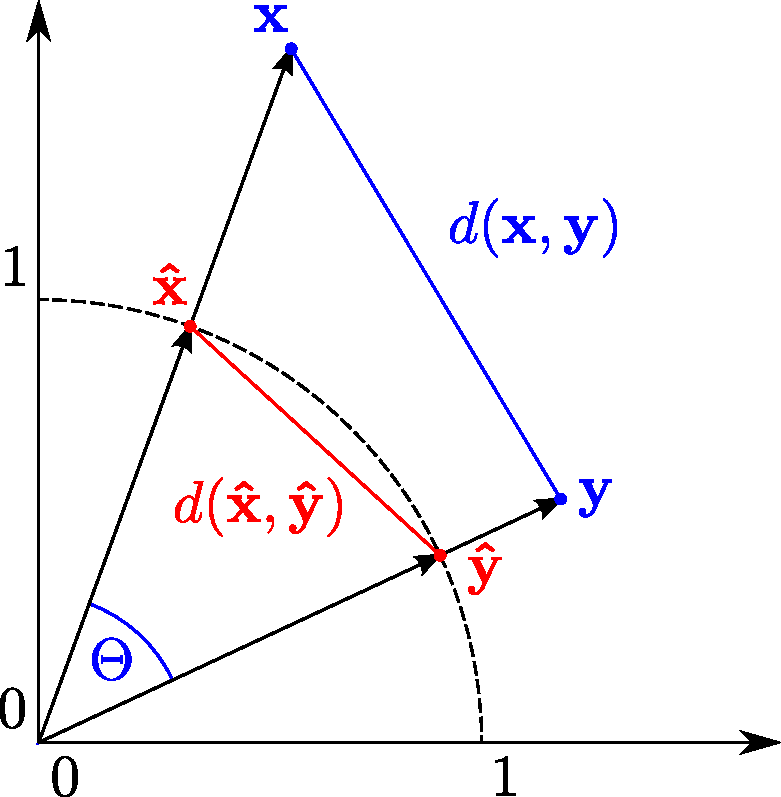
\includegraphics[width=\textwidth]{Graphics/L2.pdf}
    \end{subfigure}
    \caption[Chord Calculation Background]{\textbf{Chord Calculation Background.} The chord can be calculated with the radius similar for both vectors and the information of the angle of two vectors to the origin of the coordinate system. Since this information is not always available or sometimes expensive to calculate for a high number of vectors, the euclidean distance can be used with a L2-norm of both vectors equal to $r$ for similar results instead. To approximate cosine distance, the same calculation of euclidean distance is used with L2-norm equal to $r = 1$. To always obtain similar values of L2-norm equal to 1, L2-norm normalization is used on every vector.}
    \label{fig:L2_Normalisation_Background}
\end{figure}

\begin{equation}\label{eq:norm2}
    \begin{aligned}
        \mathbf{\hat{x}}_i = \frac{\mathbf{x}_i}{\Vert\mathbf{x}_i\Vert_2}
    \end{aligned}
\end{equation}

Calculation of chord distance $d_{\text{chord}}$ is possible when having two vectors, here as an example named as $\mathbf{x}'$ and $\mathbf{y}'$ with the same L2-norm equal to a radius $r$ of a sphere centered to the origin of the coordinate system and an angle of $\Theta'$ (\autoref{eq:chord} and \autoref{fig:L2_Normalisation_Background}). The euclidean distance $d_{\text{eucl}}$ is equal to the chord distance for the same vectors $\mathbf{x}'$ and $\mathbf{y}'$ with L2-norm of $r$.

\begin{equation}\label{eq:chord1}
    \Vert\mathbf{x}'\Vert_2 = \Vert\mathbf{y}'\Vert_2 = r \Rightarrow 
    \begin{aligned}
        d_{\text{chord}}(\mathbf{x}',\mathbf{y}') &= 2 \cdot r \sin \left(\frac{\Theta'}{2}\right)\\
        %&= 2 \cdot \frac{d_{\text{chord}}(\mathbf{x}',\mathbf{y}')}{2}\\
        %&= d_{\text{eucl}}(\mathbf{x}',\mathbf{y}')\\
        %&= \Vert\mathbf{x}' - \mathbf{y}'\Vert_2
    \end{aligned}
\end{equation}

Thus, in this project, chord distance can be calculated with the euclidean distance metric, posterior to the normalization with the L2-norm, which scales the vectors to the unit sphere.

\begin{equation}\label{eq:chord2}
    \Vert\mathbf{x}'\Vert_2 = \Vert\mathbf{y}'\Vert_2 = 1 \Rightarrow 
    \begin{aligned}
        d_{\text{chord}}(\mathbf{\hat{x}},\mathbf{\hat{y}}) &= d_{\text{eucl}}(\mathbf{\hat{x}},\mathbf{\hat{y}})\\
        &= \Vert\mathbf{\hat{x}} - \mathbf{\hat{y}}\Vert_2
    \end{aligned}
\end{equation}

The used chord distance is proportional with the initially intended to use cosine distance as shown in \autoref{eq:chord3}. Dividing the squared chord distance by 2 results in the cosine distance of the vectors.

\begin{equation}\label{eq:chord3}
    \Vert\mathbf{x}'\Vert_2 = \Vert\mathbf{y}'\Vert_2 = 1 \Rightarrow 
    \begin{aligned}  
        d_{\text{chord}}(\mathbf{\hat{x}},\mathbf{\hat{y}})^2 &= \Vert\mathbf{\hat{x}} - \mathbf{\hat{y}}\Vert_2^2\\
        &= (\mathbf{\hat{x}} - \mathbf{\hat{y}})^\top (\mathbf{\hat{x}} - \mathbf{\hat{y}})\\
        &= \mathbf{\hat{x}}^\top \mathbf{\hat{x}} - 2 \mathbf{\hat{x}}^\top \mathbf{\hat{y}} + \mathbf{\hat{y}}^\top \mathbf{\hat{y}}\\
        &= 2 - 2\mathbf{\hat{x}}^\top \mathbf{\hat{y}}\\
        &= 2 - 2 \cos(\Theta)\\
        &= 2 \cdot (1 - \cos(\Theta))\\
        &= 2 \cdot d_{\text{cos}}(\mathbf{x},\mathbf{y})
    \end{aligned}
\end{equation}

 Approximation of cosine distance by normalization with L2-norm followed by euclidean distance calculation is, thus, a possible and in this project used workaround, to overcome the impossibility to use cosine distance. 

%The default \colorbox{backcolour}{metric='euclidean'} setting was used for all following executions of \gls{HDBSCAN}, with an exception on the precalculated runs, to approximate the use of cosine distance metric as described in \autoref{sec:Normalization}. Therefore, matrix $\mathbf{X}_{\text{PCA}}$ and $\mathbf{Y}_{\text{UMAP}}$ have to be L2-norm normalized as described in \autoref{sec:Normalization} (\autoref{eq:l2_func_x} and \autoref{eq:l2_func_y}). For calculation of the linkage matrix $\mathbf{L}$, standard \gls{HDBSCAN} without $\varepsilon$ was used.

%\autoref{eq:HDB} to \autoref{eq:HDB_link_X} demonstrate the use of \gls{HDBSCAN} to calculate the linkage matrix $\mathbf{L}_{\text{PCA}}$ with matrix $\mathbf{X}_{\text{L2}}$ of \autoref{fig:Clustering_Pipeline} pathway \textsf{\textbf{1}} and was performed in the same way for $\mathbf{L}_{\text{UMAP}}$ with $\mathbf{Y}_{\text{L2}}$ of \autoref{fig:Clustering_Pipeline} pathway \textsf{\textbf{2}} \autocite{gower_minimum_1969, mcinnes_hdbscan_2017}.

% \begin{empheq}{alignat = -1}
%     &\mathbf{X}_{\text{L2}} &&= \text{NORMALIZE}_{\text{L2}}(\mathbf{X}_{\text{PCA}})\label{eq:l2_func_x}\\
%     &\mathbf{Y}_{\text{L2}} &&= \text{NORMALIZE}_{\text{L2}}(\mathbf{Y}_{\text{UMAP}})\label{eq:l2_func_y}
% \end{empheq}

% \begin{empheq}{alignat = -1}
%     &\mathbf{L}_{\text{PCA}} &&= \text{HDBSCAN}_{\text{Link}}(\mathbf{X}_{\text{L2}}, \text{min\_cluster\_size}, \text{min\_samples})\label{eq:HDB}\\
%     &&&= \text{HDBSCAN}_{\text{Link}}(\mathbf{X}_{\text{L2}}, 2, 1) \label{eq:HDB_link_X}
% \end{empheq}

Calculation of the chord distance by L2-norm normalized vectors euclidean distance is part of \glspl{HDBSCAN} mutual reachability distance calculation. The mutual reachability distance is the maximum of the chord distance and the core distances of two vectors (\autoref{eq:reach}). The core distance is the minimum radius necessary to include $k$ other vectors around a given vector. The standard setting of $k$ is five and not changed in this project \autocite{mcinnes_hdbscan_2017}. 

% \begin{empheq}{alignat = -1}
%     &d_{\text{mreach}-k}(\mathbf{x},\mathbf{y}) &&= \max \{ \text{core}_k(\mathbf{x}), \text{core}_k(\mathbf{y}), d_{\text{eucl}}(\mathbf{x},\mathbf{y}) \} \label{eq:reach}
% \end{empheq}

\begin{figure}[!hbt]
    \centering
    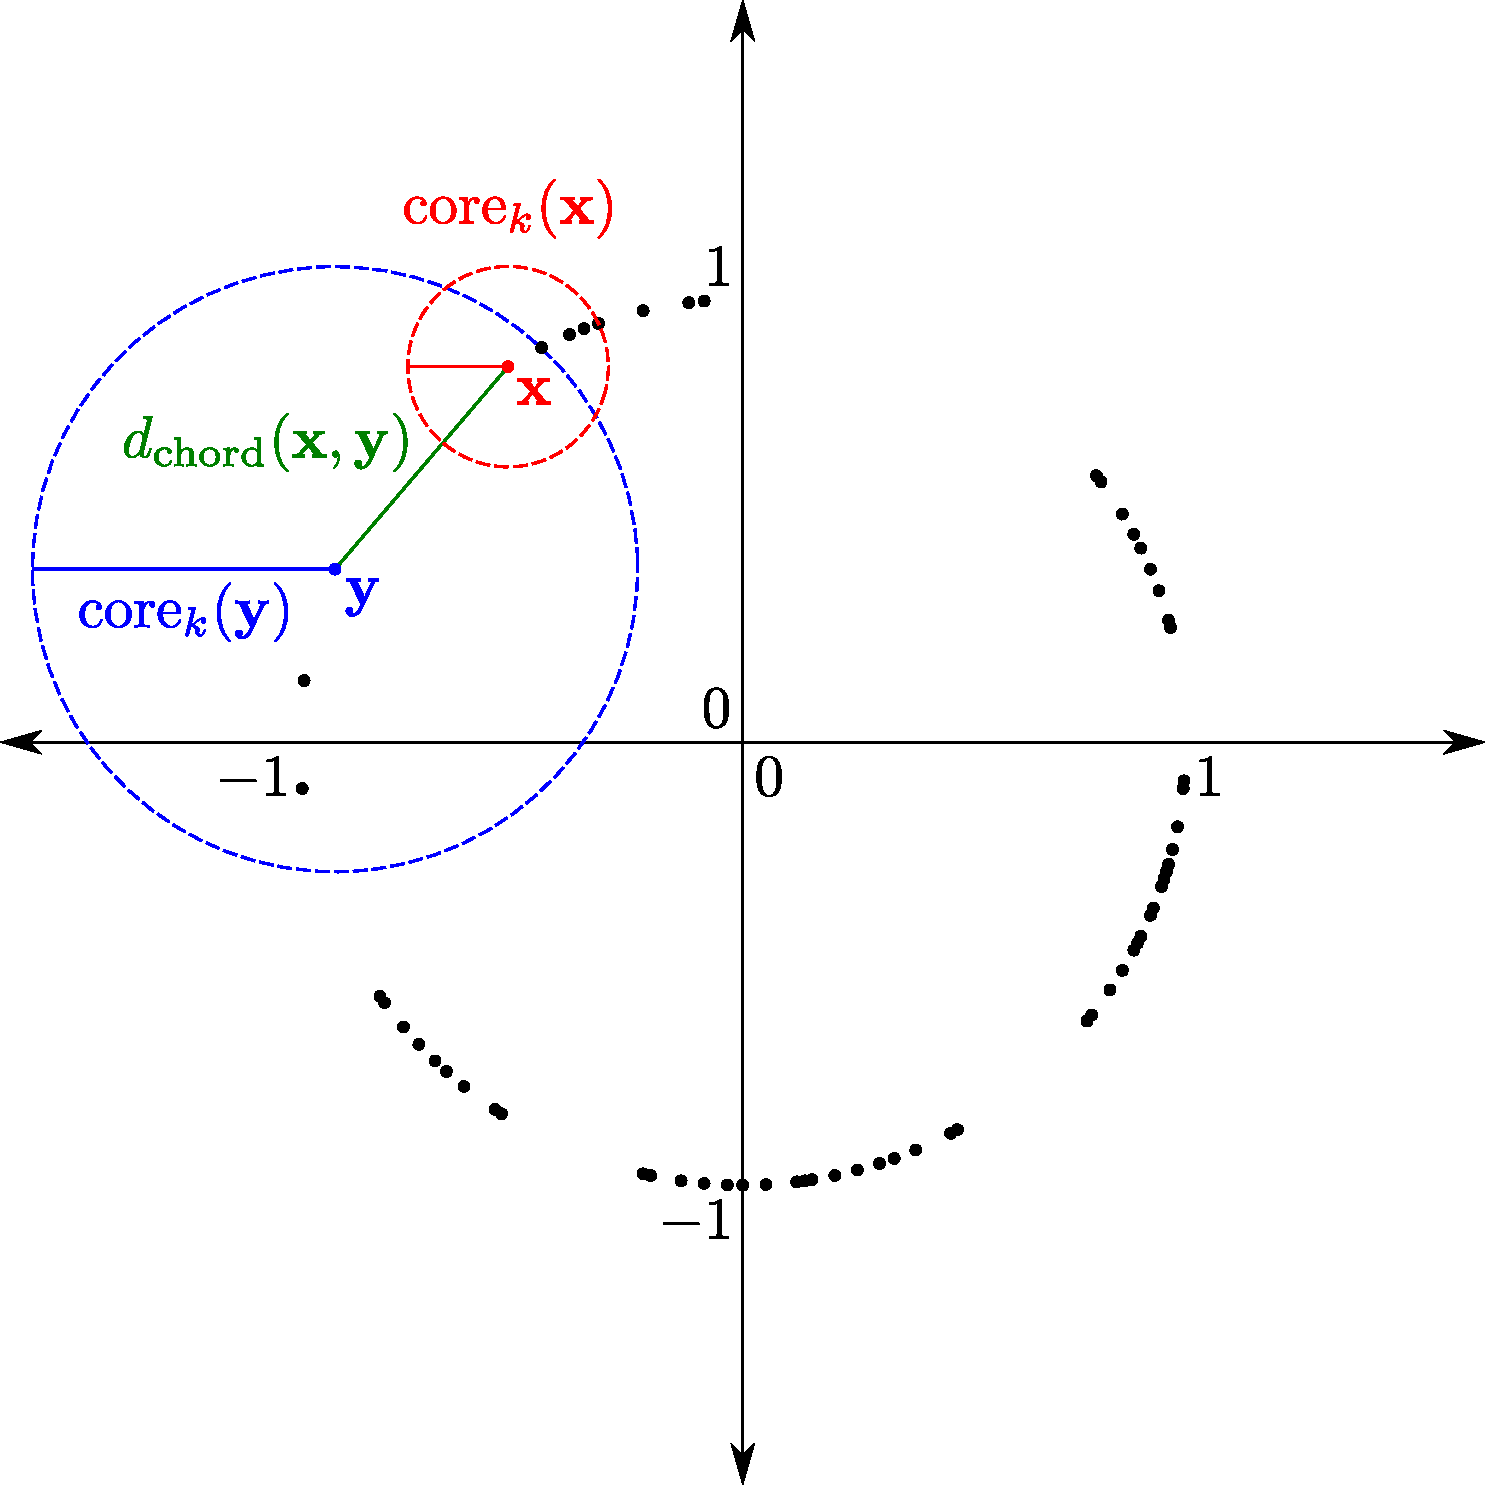
\includegraphics[width=\textwidth]{Graphics/HDB.pdf}
    \caption[Mutual Reachability Calculation]{\textbf{Mutual Reachability Calculation.} A low dimension representation of the calculation \gls{HDBSCAN} performed in this project. To calculate the mutual reachability distance, a radius is measured necessary to include the next five points, as example for vector $\mathbf{x}$ in blue and $\mathbf{y}$ in red. The euclidean distance between these vectors is then calculated and compared to the radii. The maximum of both radii and the euclidean distance is the mutual reachability distance (\autoref{eq:reach}).}
    \label{fig:HDB}
\end{figure}


\begin{figure}[!hbt]
    \centering
    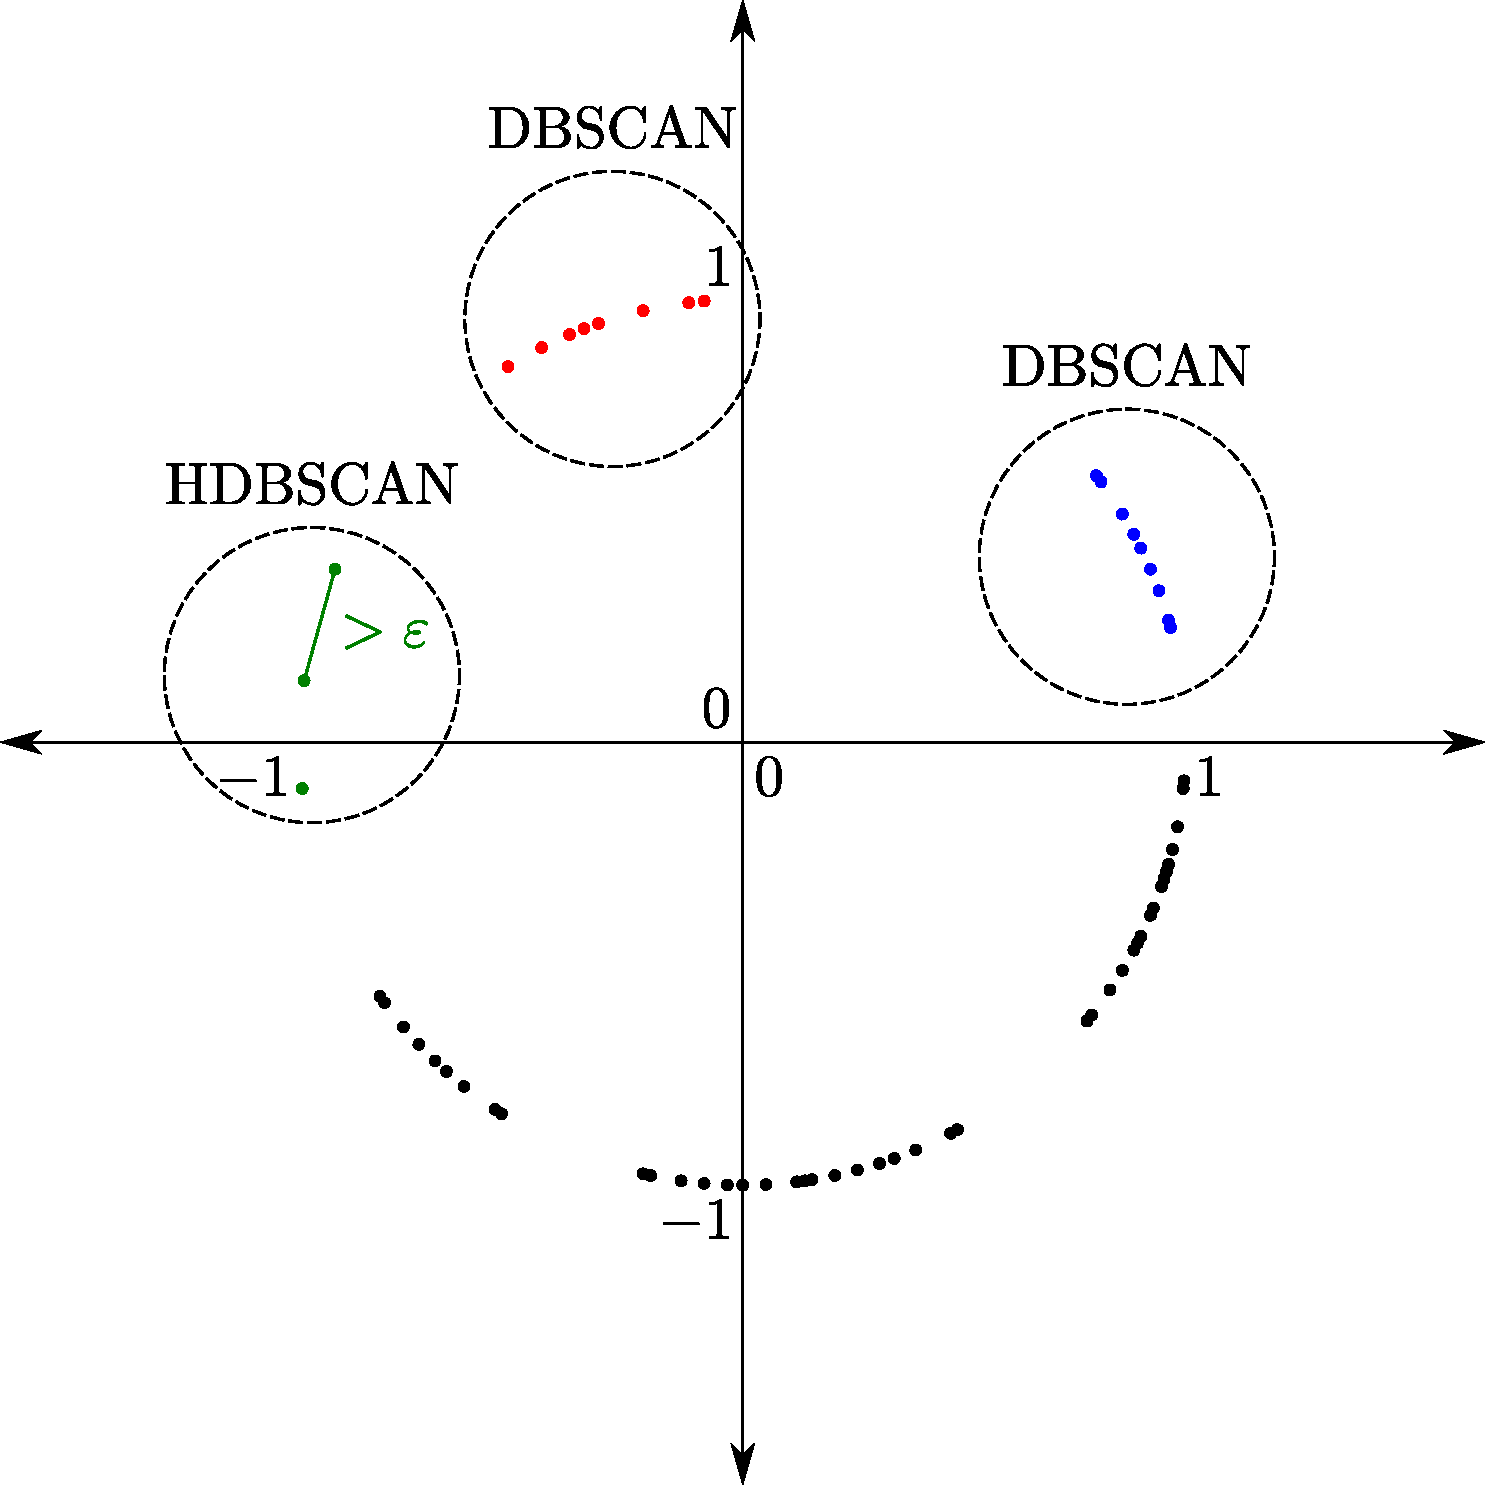
\includegraphics[width=\textwidth]{Graphics/Hybrid.pdf}
    \caption[Hybrid Clustering Threshold]{\textbf{Hybrid Clustering Threshold.} The hybrid clustering differentiate between clusters where points are connected by distances smaller and higher than $\varepsilon$. When the distance is smaller, the \gls{DBSCAN} algorithm is used and clusters are calculated based on this threshold value $\varepsilon$ by combining points with less distance. For single points, having no point in reachable distance and, therefore, impossible to be clustered by \gls{DBSCAN}, other than single sequence cluster, \gls{HDBSCAN} is used to builds cluster with higher threshold if appropriate. The graphic is based on \glqq Combining HDBSCAN* with DBSCAN\grqq{} in the \href{https://hdbscan.readthedocs.io/en/latest/api.html}{API} adapted to the calculations in this project, as two dimensional example.}
    \label{fig:Hybrid}
\end{figure}

To find an appropriate value for $\varepsilon$, two different methods were used and compared (\autoref{fig:Clustering_Pipeline} pathway \textsf{\textbf{3}} and \textsf{\textbf{4}}. Using the first method, the \gls{DBCV} exploration in \autoref{fig:Clustering_Pipeline} \textsf{\textbf{G}}, execution of \gls{HDBSCAN} was repeated with different settings for $\varepsilon$ and compared by the \gls{DBCV} to find the value of $\varepsilon$ that maximizes the \gls{DBCV} \autocite{moulavi_density-based_2014}. For these repeated executions of \gls{HDBSCAN}, \colorbox{backcolour}{gen\_min\_span\_tree=True} setting was also necessary, to be able to calculate the \gls{DBCV} with the minimum spanning tree (\autoref{eq:DBCV_X}) \autocite{moulavi_density-based_2014, gower_minimum_1969}. The exploration was executed for $\mathbf{X}_{\text{L2}}$ and $\mathbf{Y}_{\text{L2}}$ to find the optimal $\varepsilon_{\text{PCA}}$ and $\varepsilon_{\text{UMAP}}$.

% \begin{empheq}{alignat = -1}
%     &\max_{\substack{0 \leq \varepsilon}} \left(\text{HDBSCAN}_{\text{DBCV}}(\mathbf{X}_{\text{L2}}, 2, 1, \varepsilon)\right) = \text{HDBSCAN}_{\text{DBCV}}(\mathbf{X}_{\text{L2}}, 2, 1, \varepsilon') \Rightarrow \varepsilon' = \varepsilon_{\text{PCA}} \label{eq:DBCV_X}
% \end{empheq}

Using the second method, the optimal value for $\varepsilon_{\text{UMAP'}}$ and $\varepsilon_{\text{PCA'}}$ were calculated using the Kneedle Algorithm \autoref{sec:Kneedle} \autocite{halko_finding_2010}.

With the optimal values for $\varepsilon$ found by \gls{DBCV} exploration and the Kneedle Algorithm, as well as with the matrix for the \gls{UMAP} settings and the one for the \gls{PCA} settings, \gls{HDBSCAN} with the hybrid clustering setting was executed four times. Each execution resulted in the mathematical sequence of cluster names $N$ related to the sequence of genomic sequences $S$ (\autoref{eq:HDB_cluster_PK} to \autoref{eq:HDB_cluster_UD}) (\autoref{fig:Clustering_Pipeline} \textsf{\textbf{H}}) \autocite{mcinnes_hdbscan_2017, malzer_hybrid_2020}. To sum it up, with the \acrshort{UMAP}/\acrshort{DBCV} method, the cluster name of the first genomic sequence of $S$ is the first element of mathematical sequence $N_{\text{UMAP}}$. 

% \begin{empheq}{alignat = -1}
%     &N_{\text{PCA}} &&= \text{HDBSCAN}_{\text{Hybrid}}(\mathbf{X}_{\text{L2}}, 2, 1, \varepsilon_{\text{PCA}}) \label{eq:HDB_cluster_PK}\\
%     &N_{\text{UMAP}} &&= \text{HDBSCAN}_{\text{Hybrid}}(\mathbf{Y}_{\text{L2}}, 2, 1, \varepsilon_{\text{UMAP}}) \label{eq:HDB_cluster_UK}\\
%     &N_{\text{PCA'}} &&= \text{HDBSCAN}_{\text{Hybrid}}(\mathbf{X}_{\text{L2}}, 2, 1, \varepsilon_{\text{PCA'}}) \label{eq:HDB_cluster_PD}\\
%     &N_{\text{UMAP'}} &&= \text{HDBSCAN}_{\text{Hybrid}}(\mathbf{Y}_{\text{L2}}, 2, 1, \varepsilon_{\text{UMAP'}}) \label{eq:HDB_cluster_UD}
% \end{empheq}

% Important parameters used in this project, including settings varying from the default, are listed below. All available settings with explanation are listed in the \href{https://hdbscan.readthedocs.io/en/latest/api.html}{API}.

% \begin{leftbar}
%     \textbf{hdbscan.HDBSCAN}
%     \begin{nstabbing}
%         \qquad\qquad\qquad\qquad\qquad\quad\=\kill

%         min\_cluster\_size \> [min. size of a cluster (default: 5)]\\
        
%         min\_samples \> [conservativeness of the clustering (default: None)]\\
        
%         cluster\_selection\_epsilon \> [merge clusters below the threshold (default: 0.0)]\\
        
%         gen\_min\_span\_tree \> [generate the minimum spanning tree (default: False)]\\
        
%         metric \> [metric to use for clustering (default: euclidean)]
%         %alpha \> (default: 1.0)
%     \end{nstabbing}
% \end{leftbar}

%Clustering
%DBCV mehr als 50dims abkacken bla
%Metrik
%Hybrid selection
%Needle
%Linkage matrix

\section{Kneedle Algorithm} \label{sec:Kneedle}

Calculation of $\varepsilon$ was executed by using the implementation of the Kneedle Algorithm proposed in the associated \href{https://github.com/arvkevi/kneed.git}{GitHub repository} \autocite{satopaa_finding_2011}.

Points where e.~g.~ the cost of tuning is no longer worth the loss in performance are called \glqq knees\grqq{} \autocite{satopaa_finding_2011}. These points are so to speak the balance of a given trade-off \autocite{satopaa_finding_2011}. Kneedle is an algorithm to find these point in a given system \autocite{satopaa_finding_2011}. A system could be the trade-off between cluster number and distance threshold in hierarchical clustering \autocite{gower_minimum_1969}. 

With increasing cluster number, the distance threshold of hierarchical clustering decreases \autocite{gower_minimum_1969}. This describes a decreasing curve of convex type with distance threshold on the y- and cluster number on the x-axis. The knee is the number of clusters at the point in the polynomial representation of the curve with maximal acceleration. Polynomial representation was used to find the maximum acceleration of the smoothed curve, instead of a local maximum due to a single inaccuracy. Therefore the implementation Kneed was used with \colorbox{backcolour}{curve='concave'}, \colorbox{backcolour}{direction='increasing'} and \colorbox{backcolour}{interp\_method='interp1d'} settings \autoref{fig:Clustering_Pipeline} \textsf{\textbf{I}}).

\begin{empheq}{alignat = -1}
    &n &&= \text{KNEED}(\mathbf{L})
\end{empheq}

Number of clusters $n$ was then converted in it's respective distance threshold $\varepsilon$ using the linkage matrix $\mathbf{L}$ again.

The parameters used in this project with settings varying from the default are listed below. All available settings can be fount in the \href{https://kneed.readthedocs.io/en/stable/api.html}{API}.

\begin{leftbar}
    \textbf{kneed.KneeLocator}
    \begin{nstabbing}
        \qquad\qquad\qquad\qquad\qquad\quad\=\kill

        x \> \\
        
        y \> \\
        
        curve \> (default: 'concave')\\
        
        direction \> (default: 'increasing')\\
        
        interp\_method \> (default: 'interp1d')\\
        
        online \> (default: False)\\
        
        %S \> (default: 1.0)\\
        %polynomial\_degree \> (default: 7)
    \end{nstabbing}
\end{leftbar}

